\documentclass{article}

\usepackage{multicol}
\usepackage{graphicx} %\includegraphics[width=\textwidth]{path.png}
\graphicspath{ {img/} }

\title{Regelungstechnik}
\author{Prof. Dröge}
\date{}

\begin{document}

\maketitle

\newpage
\section*{\centering **.**.2024}
Semester-Anfang muss noch nachgetragen werden

\newpage
 \section*{\centering 15.10.2024}

  x) Regelgröße:
  - die physikalische Größe, die geregelt werden soll. Das bedeutet ein physikalischer Wert in einem gewünschten Maß gehalten wird.

  w) Führungsgröße:
  -

  y) Stellgröße:
  - physikalische Größe, welche die Regelgröße auf eine gewünschte Weise beeinflusst. (Bsp. Volumen Strom)

  e) Regelabweichung:
  - Differenz = Führungsgröße - Regelgröße

  z) Störgröße:
  - Einflüsse die selbst nicht beeinflusst werden können
  - Größen, die eine eingestellte Regelung aus dem Gleichgewicht bringt.

  Regelstrecke:
  - ist das zugrunde liegende System

  Systemarten: (Eingang/Ursache - Ausgang/Wirkung)
  - Intigrator: bsp. Volumenstrom wird in Volumen aufintigriert
  - Verstärker: bsp. Hebel

\newpage
\section*{\centering 12.11.2024}
\section*{\centering 14.11.2024}
letzten zwei Vorlesungen fehlen noch (müssen wegen krankheit nachgetragen werden)

\newpage
\section*{\centering 19.11.2024}
\subsection*{Wiederholung}
\subsubsection*{Merken:}
\begin{itemize}
	\item Impulsfunktion $\delta (t)$ $\rightarrow$ Gewichtsfunktion $g(t)$
	\item Sprungfunktion $\alpha (t) _{falsche variable kann aber in den Folien nachgeschaut werden}$ $\rightarrow$ Übergangsfunktion $h(t)$
	\item (für die Rücktransformation sollte Partialbruchzerlegung sitzten)
\end{itemize}

\subsubsection*{Operationsverstärker}
(siehe Folien)

\subsubsection*{Bode-Diagram}
(siehe Folien) $\rightarrow$ Selbststudium

\subsubsection*{Übergangs- und Gewichtfunkiton}
(siehe Folien) $\rightarrow$ Selbststudium

\subsubsection*{Übergangs- und Gewichtfunkiton}
(siehe Folien) $\rightarrow$ Selbststudium

\newpage
\subsection*{Teil 2 - Der Regler}
\subsubsection*{Der PID-Regler: der linearer Regler}
PID $\rightarrow$ besteht aus den drei basis Übertragungsgliedern \\
Warum PID und nicht PT1 etc.?: PT1/ PT2 sind langsamer als der P-Anteil des PID \\

Nomenklatur lernen: 
\begin{itemize}
	\item Sprungantwort $\rightarrow$ Übergangsfunktion
	\item Eingangssignal $x_e(t)$ $\rightarrow$ Regel-Abweichung
	\item Ausgangssignal $x_a(t)$ $\rightarrow$ Stellgröße
\end{itemize}

\[
G(s) = V(1+ \frac{1}{sT_N}+ sT_V)
\]
V = Verstärkung
\begin{multicols}{3}
	P-Anteil: lorem $\rightarrow$  1

	\columnbreak
	I-Anteil: Intigration $\rightarrow$ $\frac{1}{sT_N}$

	\columnbreak
	D-Anteil: Differentation $\rightarrow$ $sT_V$ \\
	(Sprungänderung ist im Einschaltmoment unendlich)
\end{multicols}
\begin{center}
	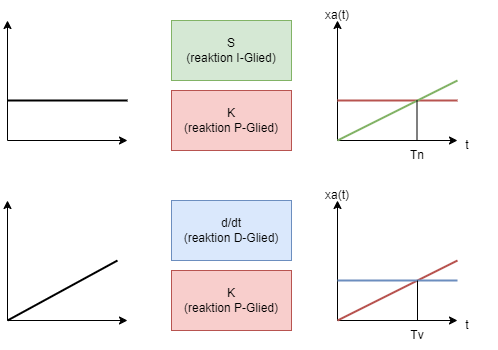
\includegraphics[width=0.6\textwidth]{19_11_2024_reglungstechnik.png}
	% 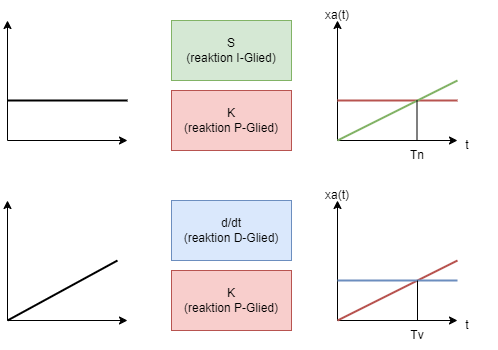
\includegraphics[width=0.5\textwidth]{19_11_2024_reglungstechnik.png}
\end{center}

Typische Anwendung der Glieder: 
\begin{multicols}{3}
	P-Regler nehmen \\
	weil?

	\columnbreak
	PI-Regler \\
	falls P nicht möglich \\
	weil?

	\columnbreak
	PID-Regler \\
	falls PI nicht möglich \\
	weil?
\end{multicols}


\newpage
\section*{\centering 21.11.2024}
\subsection*{Standardregelkreis}
Regelkreis nach DIN 19226 \\
(Grafik im Script zu finden und bereits angefangen)

\subsection*{Führungs und Störverhalten (Thema 11)}
Führungsverhalten: Wie reagiert der Regelkreis auf eine Änderung der Führungsgröße (w(t))? \\
Störverhalten: Wie reagiert der Regelkreis auf eine Änderung der Störgröße (z(t))? \\
(Grafik im Script zu finden und bereits nachgebastelt)

\subsubsection*{Berechnung der Regelgröße in Abhängigkeit der Führungsgröße}
$w(s) \rightarrow x(s)$
\[
X(s)=(W(s)-X(s)) * G_0(s)
\]
$G_0(s)=\frac{X(s)}{E(s)} = \frac{X(s)}{W(s)-X(s)}$
\[
X_W(s)=\frac{G_0(s)}{1+G_0(s)} * W(s)
\]
\[
G_{WX}(s)=\frac{X(s)}{W(s)} = \frac{G_0(s)}{1+G_0(s)}
\]

\subsubsection*{Berechnung der Regelgröße in Abhängigkeit der Führungsgröße}
$w(s) \rightarrow \epsilon(s)$ (oder auch E(s))
\[
E(s)=W(s)-X(s); X(s)=E(s)*G_0(s)
\]
\[
E(s)=W(s)-(E(s)*G_0(s))
\]
\[
E_W(s)=\frac{1}{1+G_0(s)}*W(s)
\]
\[
G_{WE}(s)=\frac{E(s)}{W(s)}=\frac{1}{1+G_0(s)}
\]

\subsubsection*{Berechnung der Regelgröße in Abhängigkeit der Störgröße}
$z(s) \rightarrow x(s)$
\[
X(s)=-X(s)*G_0(s)+Z(s)
\]
\[
X_Z(s)=\frac{1}{1+G_0(s)}*Z(s)
\]
\[
G_{ZX}(s)=\frac{X_Z(s)}{Z(s)}=\frac{1}{1+G_0(s)}
\]

\subsubsection*{Berechnung der Regelabweichung in Abhängigkeit der Störgröße}
$z(s) \rightarrow \epsilon(s)$ (oder auch E(s))
\[
E(s)=-X(s); X(s) = E(s) * G_0(s)+Z(s)
\]
\[
E(s)=-(E(s)*G_0(s)+Z(s))
\]
\[
E_Z(s)=-\frac{1}{1+G_0(s)}*Z(s)
\]
\[
G_{ZE}(s)=\frac{E_Z(s)}{Z(s)}=-\frac{1}{1+G_0(s)}
\]

\subsubsection*{Kombination von Störungs- und Führungsverhalten}
Führ die Formelsamlung: (Graftk/Zusammenfassung im Script zu finden) \\
Addition/Überlagerung von Signalen dürfen in linearen Systemen vollzogen werden.


\subsection*{Einstellregel (Thema 15)}
Wie stellt man einen Reglner ein? \\
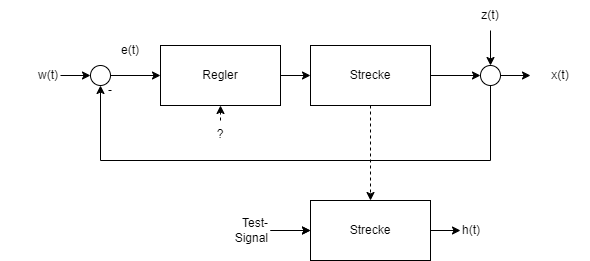
\includegraphics[width=\textwidth]{2024_11_21_Wie_stelle_ich_einen_Regler_ein.png}
(weitere Grafik im Script)\\
\begin{itemize}
	\item $T_U$ ist eine Erstatz tot-Zeit
	\item $T_G$ ist eine Ersatz-Zeit-Konstante
\end{itemize}
Zwei Varianten weil eine Regelstrecke mit I-Anteil (ohne Ausgleich) ist nicht begrentzt \\
(rest ist im Script zu finden)



\end{document}









